% Created 2018-04-23 Mon 07:58
% Intended LaTeX compiler: pdflatex
\documentclass[10pt]{beamer}
\usepackage[utf8]{inputenc}
\usepackage[T1]{fontenc}
\usepackage{graphicx}
\usepackage{grffile}
\usepackage{longtable}
\usepackage{wrapfig}
\usepackage{rotating}
\usepackage[normalem]{ulem}
\usepackage{amsmath}
\usepackage{textcomp}
\usepackage{amssymb}
\usepackage{capt-of}
\usepackage{hyperref}
\usetheme{Boadilla}
\author{ECON 420: Game Theory}
\date{Spring 2018}
\title{Continuous Strategies and Rationalizability}
\usecolortheme{seagull}
\usefonttheme[onlylarge]{structurebold}
\usefonttheme[onlymath]{serif}
\setbeamerfont*{frametitle}{size=\normalsize,series=\bfseries}
\setbeamertemplate{navigation symbols}{}
\setbeamertemplate{itemize item}[triangle]
\setbeamertemplate{footline}{}
\setbeamertemplate{enumerate items}[default]
\hypersetup{
 pdfauthor={ECON 420: Game Theory},
 pdftitle={Continuous Strategies and Rationalizability},
 pdfkeywords={},
 pdfsubject={},
 pdfcreator={Emacs 25.2.2 (Org mode 9.1.6)}, 
 pdflang={English}}
\begin{document}

\maketitle


\begin{frame}[label={sec:org7b1ebf7}]{}
\alert{Announcements}
\begin{itemize}
\item Reading: Chapter 5 and 6
\item Homework due next Monday
\item Midterm exam next Wednesday
\end{itemize}
\end{frame}


\begin{frame}[label={sec:org4df1834}]{}
\alert{Continuous strategies}
\begin{itemize}
\item So far: Games with \emph{discrete} strategies
\begin{itemize}
\item Choosing from a finite set of actions
\end{itemize}
\item Many games have many (or infinite) available actions
\item Can we generalize the notion of \emph{best response} to these settings?
\end{itemize}
\end{frame}


\begin{frame}[label={sec:orgf715342}]{}
\alert{Price-setting game}
\begin{itemize}
\item Suppose there are two competing restaurants (they make only one dish)
\item Both firms must choose their prices \(p_1\) and \(p_2\)
\item The number of dishes each restaurant sells is \(Q_i = 44 - 2p_i + p_j\)
\begin{itemize}
\item After a price change, half of your usual customers will leave to go to the other restaurant
\end{itemize}
\item The dishes cost \$8 to make for each restaurant
\item Which price should each restaurant choose?
\end{itemize}
\end{frame}

\begin{frame}[label={sec:org8b7b291}]{}
\alert{Best response}
\begin{itemize}
\item Profit depends on the pricing choice of the other firm
\item Restaurants try to profit maximize given the price that they think the other will choose
\item This pricing strategy is the \emph{best response} of the restaurant
\end{itemize}
\end{frame}

\begin{frame}[label={sec:orge227bb5}]{}
\alert{Can the restaurants do better?}
\begin{itemize}
\item Suppose an outside company buys both restaurants
\item The firm is now a monopolist, chooses one price for both locations
\item What is the optimal price? What are the profits?
\end{itemize}
\end{frame}

\begin{frame}[label={sec:org200e6be}]{}
\alert{Collusion}
\begin{itemize}
\item The pricing game is a form of a prisoners' dilemma (with continuous strategies)
\item The firms could cooperate to split the monopolist profits
\item But each can do better (individually) by choosing something \emph{other} than the monopolist price
\item Cooperation is \emph{never} a best response
\end{itemize}
\end{frame}

\begin{frame}[label={sec:org9d95879}]{}
\alert{Limitations of NE?}

Example:
\begin{itemize}
\item Player A: Chooses "Up" or "Down"
\item Player B: Chooses "Left" or "Right"
\item Payoffs (A, B):
\begin{itemize}
\item Up, Left: (2 chocolates, 2 chocolates)
\item Up, Right: (1 chocolates, 1 chocolates)
\item Down, Left: (3 chocolates, 2 chocolates)
\item Down, Right: (50\% penalty on midterm, 1 chocolate)
\end{itemize}
\end{itemize}
\end{frame}

\begin{frame}[label={sec:org73f2a65}]{}
\alert{Why might we not see a NE?}
\begin{itemize}
\item Often, player A won't choose Down, because it is risky
\item Why is it risky?
\begin{itemize}
\item A might think B doesn't like chocolate
\item A might be concerned the B will try to "spite" them
\end{itemize}
\item These options might mean that the game is \emph{misspecified}
\begin{itemize}
\item A has uncertainty about B's payoffs
\end{itemize}
\end{itemize}
\end{frame}

\begin{frame}[label={sec:orge8b05d8}]{Example}
\begin{center}
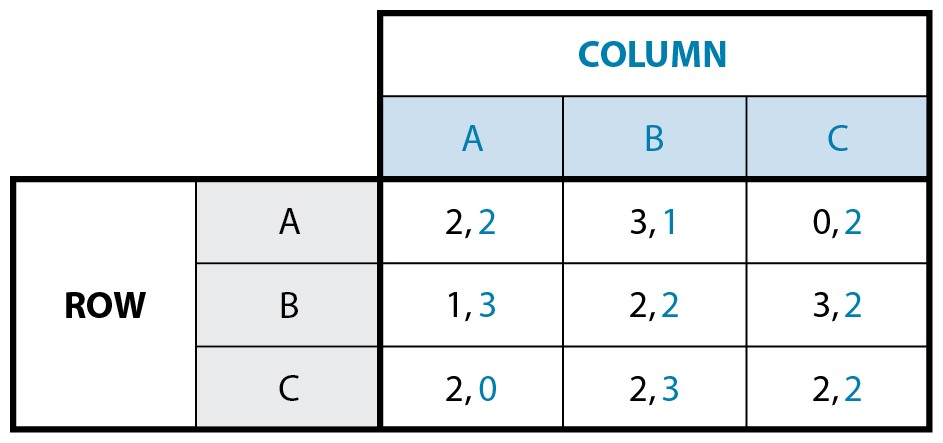
\includegraphics[width=.75\textwidth]{./img/GAMES4_FIG05.03.jpg}
\end{center}
\end{frame}

\begin{frame}[label={sec:orgbf74e97}]{}
\alert{Rationalization}
\begin{itemize}
\item Suppose games are properly specified
\item Nash equilibrium:
\begin{itemize}
\item The choice of each player is their best response given their beliefs about what the other players are doing
\item The beliefs are accurate
\end{itemize}
\item Does this mean that purely rational players will achieve the NE?
\end{itemize}
\end{frame}

\begin{frame}[label={sec:org6573edd}]{}
\begin{center}
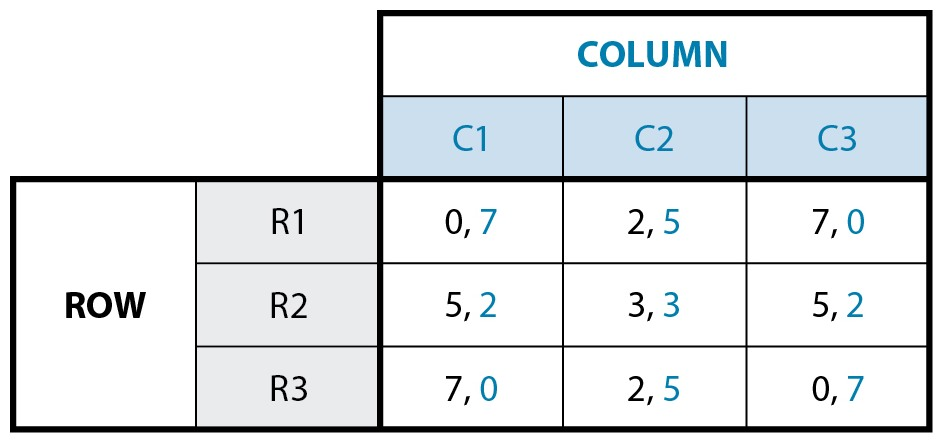
\includegraphics[width=.75\textwidth]{./img/GAMES4_FIG05.05.jpg}
\end{center}
\end{frame}

\begin{frame}[label={sec:orgd141ca3}]{}
\alert{Rationalizability}
\begin{itemize}
\item Multiple outcomes can be supported by rational "chains" of thought
\begin{itemize}
\item Not necessarily NE
\end{itemize}
\item But not \emph{every} outcome is supported by rationality
\item For instance: It is never rational to play a strategy that is \emph{never a best response}
\end{itemize}
\end{frame}

\begin{frame}[label={sec:orgb3faa36}]{}
\begin{center}
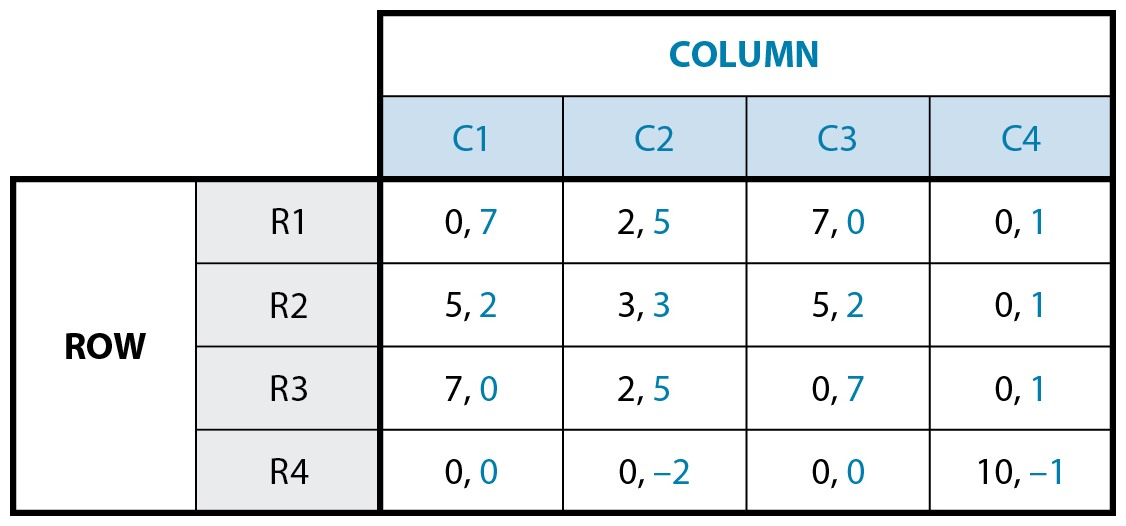
\includegraphics[width=.75\textwidth]{./img/GAMES4_FIG05.06.jpg}
\end{center}
\end{frame}

\begin{frame}[label={sec:org6763a6d}]{}
\alert{Rationalizability}
\begin{itemize}
\item Note: Not all strategies that are never a best response are dominated by some other strategy
\item Sometimes rationalizability can lead to a NE (but not always)
\end{itemize}
\end{frame}
\begin{frame}[label={sec:org5bfcd1d}]{}
\alert{Cournot competition}
\begin{itemize}
\item Suppose there are two fishing boats that choose how many fish to catch each day
\item The local fish market buys the fish for a price \(P=60-Y\)
\item Boat one has costs of 30 per fish and boat 2 has costs 36 per fish
\end{itemize}
\end{frame}
\end{document}